\section{Architectures se basant sur ces partitionnements}

\subsection{Principales problématiques}
Bien que la première partie de ce rapport ait exposé des pistes de résolution du problème de la charge d'une seule machine, d'autres problématiques complexes se posent sur la gestion d'un serveur de jeu vidéo.

\paragraph{Division du monde entre les machines\\}
Répartir les données n'est pas forcément simple, surtout en ce qui concerne la gestion de la cohérence aux frontières.
En effet, une action de joueur peut avoir une interaction sur plusieurs objets du monde du jeu en même temps, ces objets pouvant être gérés par des serveurs différents à la frontière.
Il faut également faire attention aux transferts de joueurs entre serveurs pendant la zone d'overlap.
Pour éviter de générer beaucoup de frontières, on préférera par exemple donner des zones adjacentes à une même machine car la gestion de la cohérence se fera en interne.
Comme présenté dans la partie sur le zoning, celui-ci peut être dynamique.

\paragraph{Cohérence du monde\\}
Lors d'extrapolation (prédiction) de la part du client, l'état global du jeu stocké peut diverger de l'état réel.
Cela crée donc des incohérences qu'il faut gérer pour savoir lequel des deux état est correct.
Dans le cas de plusieurs machines, il faut aussi savoir dans quel ordre effectuer les actions des joueurs pour rester dans un état cohérent.
Il faut donc gérer les verrous pour éviter les modifications concurrentes des mêmes objets.
Dans les zones de chevauchement, ces verrous sont plus important car les objets sont gérés sur au moins deux machines.

\paragraph{Tolérance aux fautes\\}
Lorsqu'une machine devient indisponible (à cause d'un crash ou d'un problème réseau), le jeu doit pouvoir continuer à s'exécuter sans interruption de service pour fournir une bonne expérience au joueur.
Un arrêt du jeu non commandé par le joueur réduit grandement l'immersion.

\paragraph{Latence\\}
Le problème de la latence est très complexe.
Premièrement, il faut qu'un joueur disposant d'une connexion lente ne soit pas désavantagé par rapport à un joueur disposant d'une connexion rapide pour des raisons de jouabilité (il faut que le jeu reste ``fair'').
Deuxièmement, il faut que le serveur fournisse au client assez rapidement l'état du jeu pour que les données restent pertinentes dans le contexte du jeu.
Dans un FPS, la position d'un autre joueur est une donnée très importante ayant une durée de vie courte (si l'ennemi a bougé entre temps cela est suffisant pour le ``rater'') et un joueur ne recevant pas suffisamment de mises à jour se retrouvera désavantagé.
Les parties graphiques de chaque client les plus lents seront donc obligées de prédire et d'extrapoler entre les deux mises à jour (dead reckogning).

\paragraph{Gestion de la triche\\}
Ce problème est plus important dans un MMOG que dans d'autres types de jeux car le monde est persistant et un désavantage lié à la triche, qui restait cantonné à la partie en cours pour un jeu normal, devient permanent.
Il faut donc pouvoir authentifier quel comportement est correct ou non pour un joueur.
La triche peut avoir lieu à plusieurs niveaux~\cite{low_latency_and_cheat_proof_ordering_p2p}~:

\begin{itemize}
	\item Niveau protocole : ajout de délai à l'envoi de paquet, falsification d'horodatage (timestamp), omission de certains messages, envoi de versions différentes à différentes personnes (production d'incohérence), utilisation de données hors de notre champ normal d'intérêt...
	\item Niveau logique du jeu : modification de données côté client, envoi de déplacements incorrects...
	\item Niveau application : modification du code du jeu pour gagner des avantages (par exemple rendre le rendu client des murs transparents pour savoir où se situent les ennemis).
\end{itemize}

\paragraph{Dimensionnement du nombre de machines\\}
Lors de la création du serveur du jeu vidéo, il faut faire attention à ne pas trop le surdimensionner pour éviter les coûts et ne pas perdre une grande partie des bénéfices avec des machines sous-utilisées.
De nombreux serveurs de jeu sont surdimensionnés pour absorber la charge lors de grandes affluences mais restent vides une majeure partie du temps, par exemple vers 7h du matin (voir \textsc{Figure}~\ref{fig:player_day_evol}).
Dimensionner correctement le serveur permet de minimiser le nombre de machines utilisées pour éviter que les serveurs soient à moitié vides.

\subsection{Architecture Client-Serveur}
\begin{figure}[b!]
		\centering
		\begin{subfigure}[t]{0.3\textwidth}
			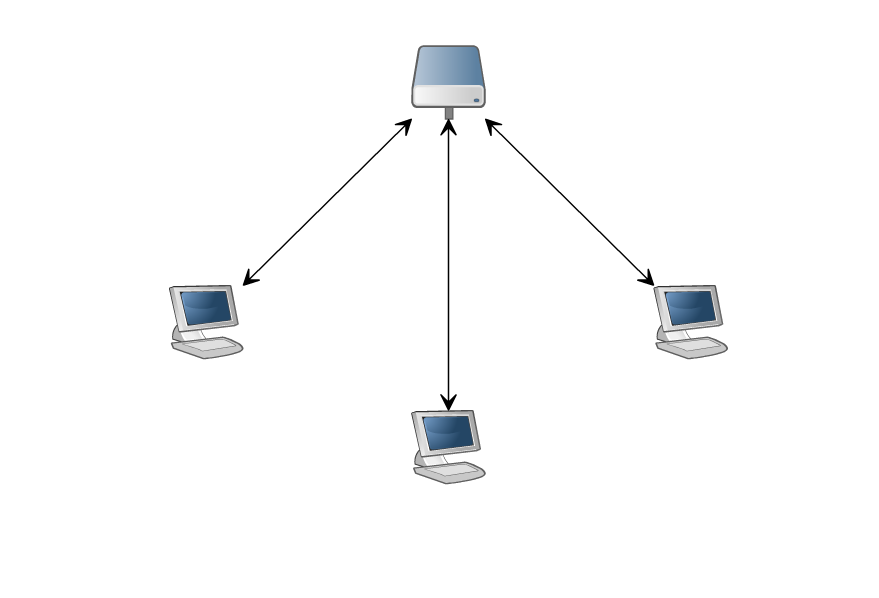
\includegraphics[width=\textwidth]{cs.png}
			\caption{Client-serveur classique}
			\label{fig:archi_cs}
		\end{subfigure}
		~
		\begin{subfigure}[t]{0.3\textwidth}
			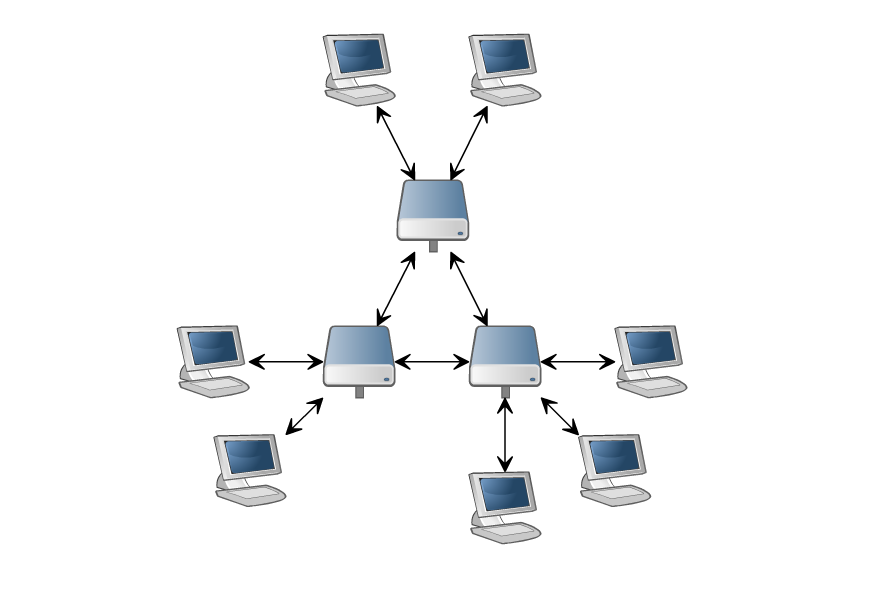
\includegraphics[width=\textwidth]{mcs.png}
			\caption{Multi-serveur}
			\label{fig:archi_mcs}
		\end{subfigure}
		~
		\begin{subfigure}[t]{0.3\textwidth}
			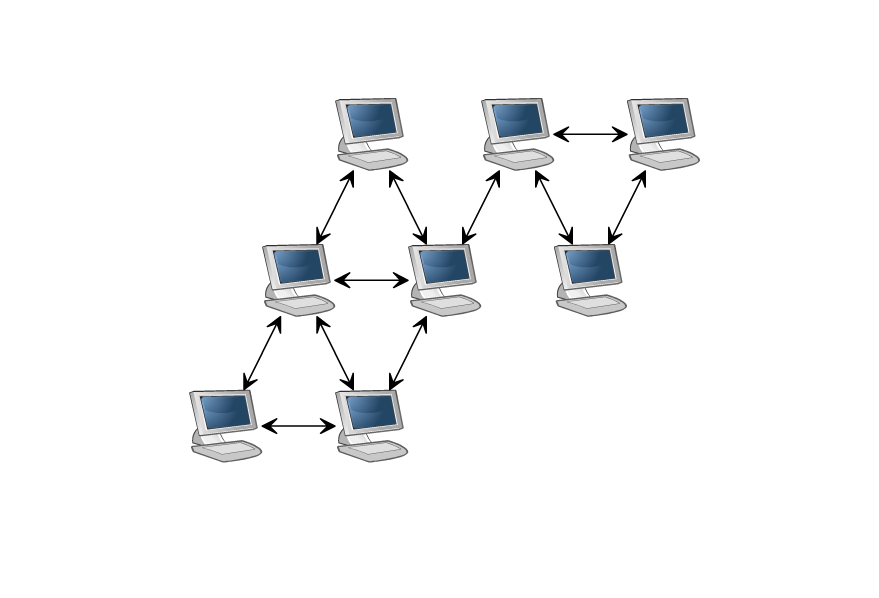
\includegraphics[width=\textwidth]{p2p.png}
			\caption{Pair-à-Pair}
			\label{fig:archi_p2p}
		\end{subfigure}
		\\[0.2cm]
	\caption{Architectures classiques}
	\label{fig:archi}
\end{figure}
Dans l'architecture client-serveur classique, le serveur est responsable de l'état global du monde, il reçoit les mises à jour de la part des clients, calcule le nouvel état et en envoie une copie aux joueurs (\textsc{Figure}~\ref{fig:archi_cs}).
La majeure partie des jeux à succès est basée sur cette architecture.
Les serveurs plus simples peuvent être déployés n'importe où, comme les serveurs de jeux de tir à la première personne ou ceux de Minecraft qui sont très nombreux.

Cette architecture peut également être basée sur de multiples machines pour des plus gros jeux tels que Second Life ou World of Warcraft (\textsc{Figure}~\ref{fig:archi_mcs}).
Ces architectures multi-serveurs se basent sur les partitionnements vus en partie II pour tenir la charge d'un MMOG.

Le serveur BigWorld~\cite{bigworld} est une architecture multi-serveurs qui utilise une grande partie des découpages de la partie précédente (voir \textsc{Figure}~\ref{fig:bigworld}).
Dans cette architecture, chacun des éléments du jeu est séparé en services (login, database...) qui sont hébergés par des machines différentes.
De plus, le monde est découpé en cellules (cell) qui sont des séparations du monde grâce à des rectangles aux côtés alignés qui sont hébergés chacun par une machine.
Comme ces séparations sont dynamiques pour assurer l'équilibrage de charge, les machines sous-utilisées peuvent être arrêtées et leur zones respectives données aux autres machines pour réduire les coûts.
Cela peut également améliorer la durée de vie des machines.

Une technique de proxy peut être mise en place pour permettre de séparer la charge réseau sur différentes machines.
Les machines proxy répliquent l'état du jeu et chacune transmet cet état à un nombre réduit de joueurs (partagé entre tous les proxys).
Ceci tire profit du fait que la connexion inter-machines (réseau local) est bien souvent plus rapide que leur connexion vers l'extérieur (internet).

Le serveur Pikko~\cite{pikko} utilise un serveur écrit en Erlang qui sert de répartiteur de charge entre toutes les machines du serveur de jeu.
C'est ce répartiteur qui décide les transferts de joueurs entre les machines et qui redirige les actions des joueurs vers la bonne machine.
Ceci permettra dans le futur MMOG Warhammer 40000 : Eternal Crusade~\cite{wh40kEC} de faire des batailles comprenant de très nombreux joueurs dans la même zone (plus de 500).
Cette technologie a été testée à l'occasion d'une démonstration nommée Tanks vs. Robots qui a permis d'atteindre un record dans le Guiness Book grâce à 1000 joueurs simultanés~\cite{tanks_vs_robots}.

\begin{figure}[b!]
	\centering
	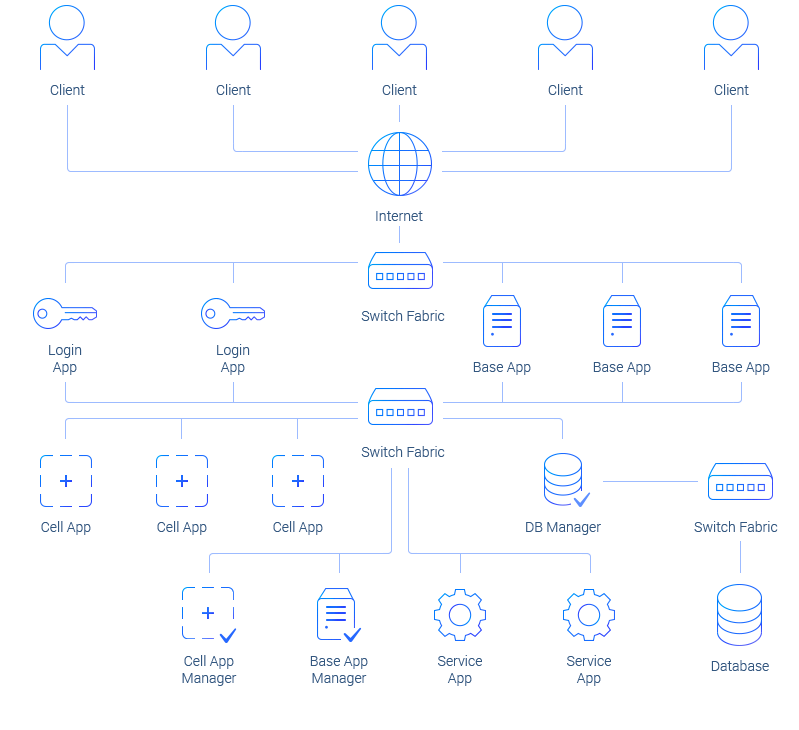
\includegraphics[width=0.7\textwidth]{bigworld.png}
	\\[0.2cm]
	\caption{Fonctionnement du Serveur Bigworld~\cite{bigworld}}
	\label{fig:bigworld}
\end{figure}

\subsection{Architecture Pair-à-Pair}
Un MMOG nécessite d'avantage de ressource pour gérer chacun des nouveaux joueurs se connectant.
Cependant, chacun des joueurs qui se connecte amène également des ressources via son ordinateur.
Les architectures Pair-à-Pair (\textsc{Figure}~\ref{fig:archi_cs}) exploitent ceci en utilisant la puissance de calcul et le réseau des clients pour effectuer les tâches qui s'exécutent normalement du côté du serveur.
Il faut alors intégrer au client du jeu toute la logique du serveur.
Comme chacun des joueurs amène ses propres ressources, le système peut théoriquement passer à l'échelle indéfiniement.

Cette architecture est la problématique la plus étudiée dans le domaine de la recherche pour les architectures de serveurs pour MMOG.
Un des premiers mondes virtuels utilisant l'architecture Pair-à-Pair est Solipsis~\cite{solipsis}.
Dans Solipsis, chaque Pair envoie les mises à jour aux autres pairs situés dans un certain rayon de visibilité.
VON/VAST~\cite{VON}~\cite{VAST} et Voronet~\cite{voronet} utilisent une approche similaire en utilisant une triangulation de Delaunay (et les diagrammes de Voronoi) pour connecter les pairs les plus susceptibles d'échanger de l'information (les plus proches dans le monde virtuel).
Ceci réduit les latences en propageant les mises à jour du monde sous forme de vague.

VoroGame~\cite{vorogame} utilise deux couches de distribution pair-à-pair : une triangulation de Delaunay pour découvrir les voisins et une DHT (table de hachage distribuée) pour stocker les objets du monde.
Colyseus~\cite{colyseus} utilise des rectangles aux bords dynamiques alignés pour répartir la charge entre les clients.

\subsection{Architectures hybrides}
Les architectures hybrides se comportent comme un mélange des deux architectures précédentes.
Des ``Super Peers'' sont élus pamis les joueurs et se comportent comme des serveurs de jeu au sein du maillage de l'architecture Pair-à-Pair.
Ces Super Peers sont choisis pamis les joueurs ayant suffisamment de puissance de calcul et une bonne connexion avec les autres~\cite{super_peer_network}.
Un système utilisant cette architecture est MOPAR~\cite{MOPAR} qui est semblable à VoroGame~\cite{vorogame} mais n'utilisant que les Super Peers pour effectuer les calculs en utilisant des zones fixes.

Cependant, comme ces Super Peers sont responsables de certaines données, il faut les choisir de manière judicieuse.
En effet, un Super Peer peut plus facilement tricher en modifiant les données dont il est le responsable.
Des algorithmes de ``confiance'' peuvent être mis en place pour retirer les joueurs soupçonnés de triches en mettant à contribution des vérifications du côté des autres pairs.
De plus, des machines d'architecture Client-Serveur peuvent faire partie du réseau pour créer une autorité de gestion de la triche.
Il faut remarquer que l'introduction de Super Peers réintroduit le problème de point de chute des architectures client-serveur dans l'architecture Pair-à-Pair~\cite{design_issues_for_p2p_mmog}.

\subsection{Le Game as a Service ou ``cloud gaming''}
Certains industriels commencent à explorer une nouvelle méthode de distribution du jeu vidéo.
Plutôt que de télécharger le client de jeu (qui peut devenir très lourd pour les jeux photoréalistes en 3D), le serveur de jeu envoie directement un flux vidéo du jeu (stream) au joueur qui renvoie en échange les entrées (input) (voir \textsc{Figure}~\ref{fig:gaas}).
Cela permet, par exemple, aux joueurs dotés d'un ordinateur peu puissant de se décharger des calculs graphiques pour exécuter le jeu dans une qualité optimale.
Le nom commercial de cette technique est le ``cloud gaming'' mais un nom correspondant mieux est ``Game as a Service'' car l'architecture nécessite du matériel spécialisé~: elle ne se situe pas chez les fournisseurs de cloud usuels.

Cette méthode, bien qu'intéressante, nécessite une très bonne connexion internet, que de nombreux joueurs ne possèdent pas.
Le service de GaaS de Nvidia (Nvidia Grid~\cite{grid}, service pour leur gamme de tablette Nvidia Shield) impose comme prérequis 40 à 60 ms de ping et 10 Mbps en téléchargement par exemple.
De plus, la charge de calcul graphique et réseau du côté serveur devient bien plus importante qu'un serveur ne partageant que l'état du jeu.
Le matériel spécialisé dans ce type de service est d'ailleurs très cher et peu performant.
Par exemple, Nvidia propose la gamme Nvidia Grid (matériel) avec le modèle K520 qui permet de fournir de 2 à 16 joueurs, en résolution 720p à 30 images par seconde, constaté neuf à 2800\$ le 13/03/2015 chez Amazon~\cite{grid_k520}.
L'investissement est donc important pour le nombre de joueurs que la carte peut fournir et la vidéo fournie n'est pas d'une qualité que l'on aurait avec une carte graphique sur un ordinateur de bureau (1080p et 60 images par seconde) sans encombrer le réseau.

Certains fournisseurs utilisent cette méthode pour diffuser du contenu en local pour l'utilisateur, pour par exemple jouer à un jeu très demandeur en ressources sur un ordinateur beaucoup moins puissant que nécessaire en utilisant la puissance d'un autre ordinateur sur le réseau local, par exemple Steam In-Home Streaming~\cite{steam_inhome}, GamingAnywhere~\cite{gaminganywhere_article} ou StreamMyGame~\cite{streammygame}.
Ceci permet par exemple de jouer sur une télévision à l'aide d'un mini-ordinateur.

\begin{figure}[t!]
	\centering
	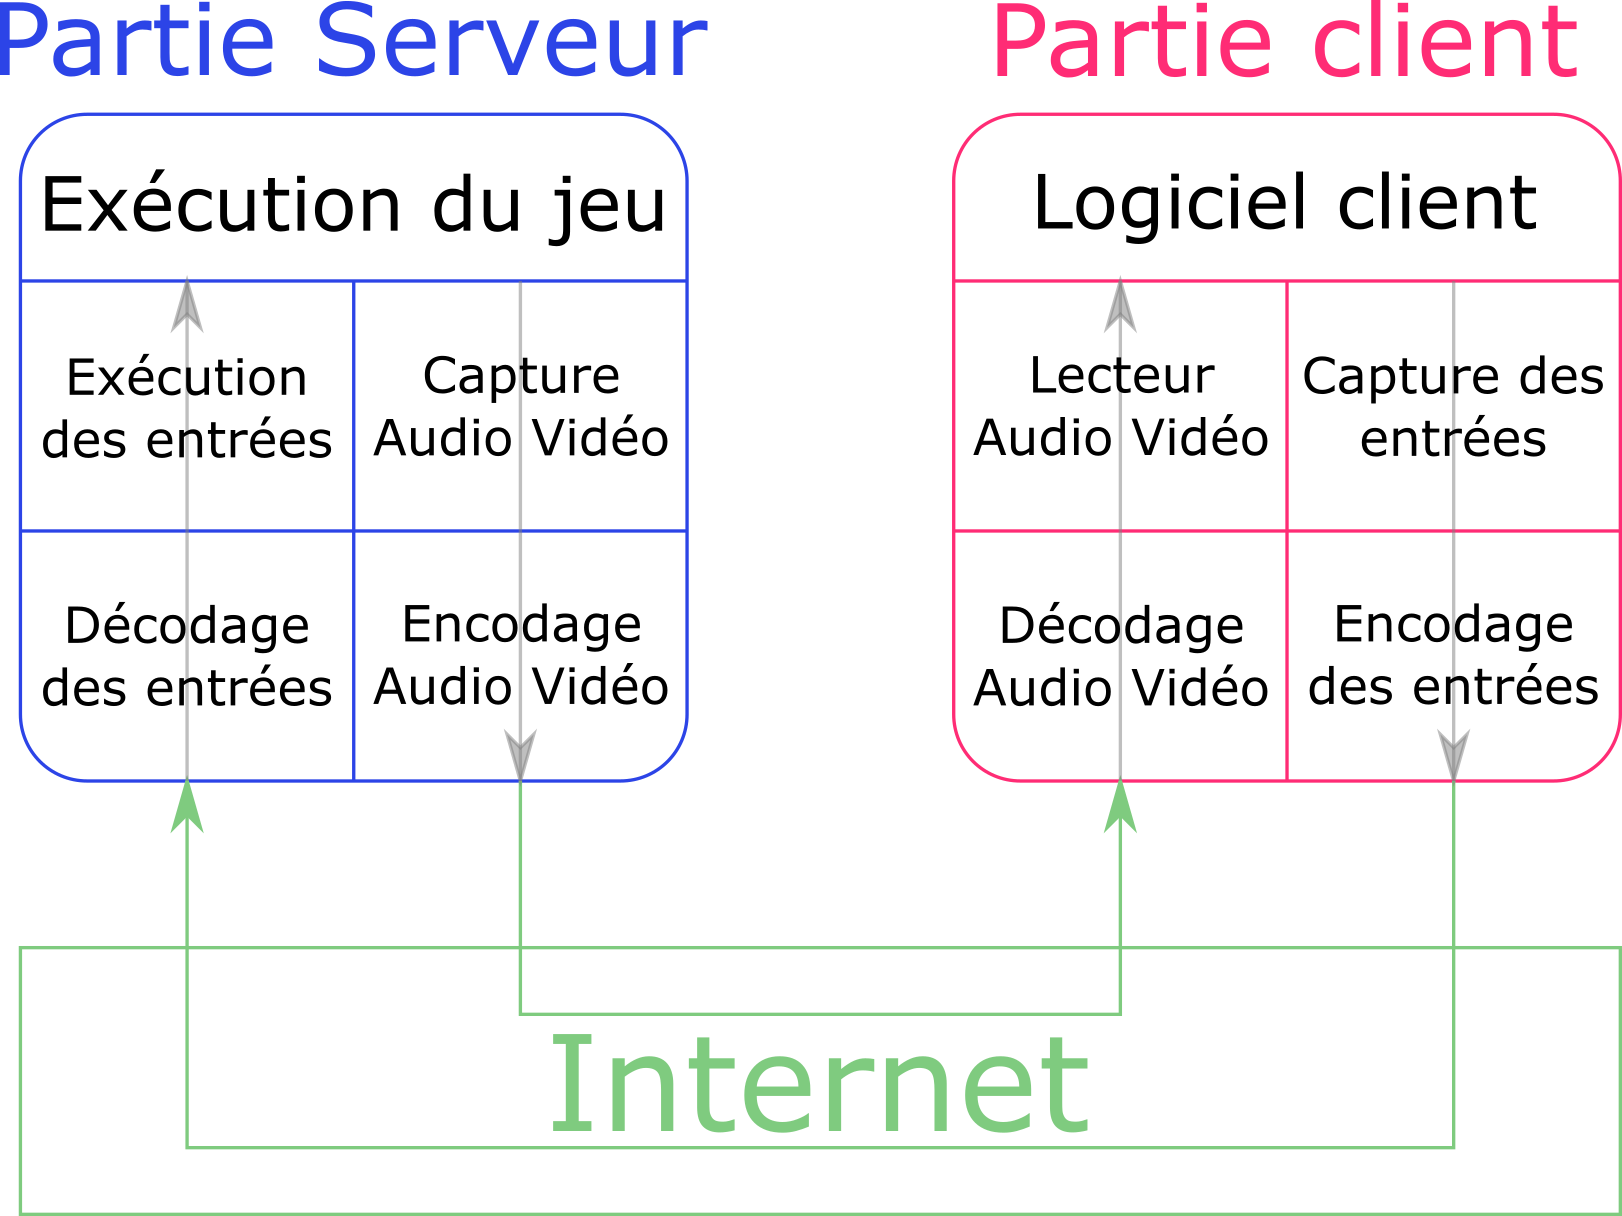
\includegraphics[width=0.5\textwidth]{gaas.png}
	\\[0.2cm]
	\caption{Fonctionnement du Game as a Service}
	\label{fig:gaas}
\end{figure}
